\documentclass[aspectratio=169,10pt]{beamer}

\usetheme{Madrid}
\usecolortheme{default}
\setbeamertemplate{navigation symbols}{}
\setbeamertemplate{footline}[frame number]

\usepackage{amsmath,amssymb,amsthm,booktabs,mathtools}
\usepackage{graphicx}
\usepackage{hyperref}
\usepackage{tikz}
\usetikzlibrary{arrows.meta,positioning,decorations.pathreplacing,arrows,automata,shapes.geometric,fit,calc}

% Semantic colors
\definecolor{positive}{HTML}{0173B2}
\definecolor{negative}{HTML}{DE8F05}
\definecolor{emphasis}{HTML}{029E73}
\definecolor{neutral}{gray}{0.55}
\definecolor{cbPurple}{HTML}{CC78BC}
\newcommand{\pos}[1]{\textcolor{positive}{#1}}
\newcommand{\con}[1]{\textcolor{negative}{#1}}
\newcommand{\HL}[1]{\textcolor{emphasis}{#1}}

\title[NeSy-MBST]{The Machine Proposes. The Proof Disposes.}
\subtitle{Neuro-Symbolic Synthesis of Formally Verified Markov Usage Models\\from Natural Language Requirements}
\author[Nathan G. et al.]{Nathan G., Jordan Chay, Jaeden Ting YiYong, Wai Phyo Hein}
\institute[Sunway University]{School of Computing and Artificial Intelligence, Sunway University\\
\small{Subang Jaya, Malaysia}}
\date{2025}

\begin{document}

% ─── TITLE ───────────────────────────────────────────────────────────────────
\begin{frame}
  \titlepage
\end{frame}

% ─── OUTLINE ─────────────────────────────────────────────────────────────────
\begin{frame}{Outline}
  \tableofcontents[hideallsubsections]
\end{frame}

% ─── SECTION 1: MOTIVATION ───────────────────────────────────────────────────
\section{Motivation \& Problem}

\begin{frame}{The MBST Bottleneck}
  \begin{columns}[T]
    \column{0.55\textwidth}
      \textbf{Model-Based Statistical Testing (MBST)}
      \begin{itemize}
        \item Replaces ad-hoc testing with \pos{probabilistic test generation}
        \item Markov chain usage model encodes operational profile
        \item Enables statistical reliability certification
      \end{itemize}
      \vspace{0.4em}
      \textbf{\con{The blocking problem}}
      \begin{itemize}
        \item Manual model construction: \con{labor-intensive, expert-only}
        \item Confined MBST to aerospace, medical, telecom niches
        \item Natural-language requirements $\to$ verified state machines: \con{no automated path}
      \end{itemize}
    \column{0.42\textwidth}
      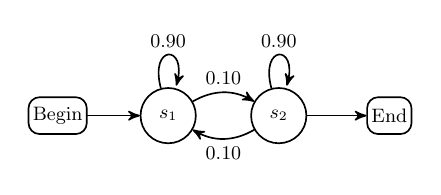
\begin{tikzpicture}[->, >=stealth', auto, semithick, node distance=1.8cm, scale=0.78, transform shape]
        \tikzstyle{state}=[circle, draw, minimum size=0.9cm, inner sep=0pt, font=\small]
        \tikzstyle{terminal}=[rectangle, rounded corners, draw, minimum size=0.6cm, inner sep=2pt, font=\small]
        \node[terminal]                (begin) {Begin};
        \node[state, right of=begin]   (A)     {$s_1$};
        \node[state, right of=A]       (B)     {$s_2$};
        \node[terminal, right of=B]    (end)   {End};
        \path (begin) edge node {} (A);
        \path (A) edge [loop above] node {\small 0.90} (A);
        \path (A) edge [bend left]  node {\small 0.10} (B);
        \path (B) edge [bend left]  node {\small 0.10} (A);
        \path (B) edge [loop above] node {\small 0.90} (B);
        \path (B) edge node {} (end);
      \end{tikzpicture}
      \vspace{0.4em}
      \begin{center}\small\textcolor{neutral}{Markov chain usage model}\end{center}
  \end{columns}
\end{frame}

\begin{frame}{Four Structural Bottlenecks of Pure-Neural Approaches}
  \begin{columns}[T]
    \column{0.48\textwidth}
      \begin{alertblock}{\con{B1: Hallucination}}
        LLMs omit edges, create impossible transitions, violate system invariants
      \end{alertblock}
      \vspace{0.3em}
      \begin{alertblock}{\con{B2: Calibration failure}}
        LLMs cannot guarantee row-stochastic $\mathbf{P}$:\\
        $\sum_j p_{ij} = 1$, $p_{ij} \geq 0$ — violated silently
      \end{alertblock}
    \column{0.48\textwidth}
      \begin{alertblock}{\con{B3: State-space explosion}}
        Finite context window $\Rightarrow$ context fragmentation on large concurrent models
      \end{alertblock}
      \vspace{0.3em}
      \begin{alertblock}{\con{B4: Structural incompleteness}}
        Recall-limited generation misses guard--action semantics of transitions
      \end{alertblock}
  \end{columns}
  \vspace{0.5em}
  \begin{center}
    \HL{$\Rightarrow$ None of these can be fixed by prompting alone}
  \end{center}
\end{frame}

% ─── SECTION 2: RESEARCH QUESTIONS ───────────────────────────────────────────
\section{Research Questions}

\begin{frame}{Research Questions}
  \begin{block}{RQ1 — Structural Fidelity}
    Can automated neuro-symbolic construction achieve $F_1 \geq 0.90$ for safety-critical test generation, without manual modelling?
  \end{block}
  \vspace{0.2em}
  \begin{block}{RQ2 — Fault-Detection Coverage}
    Does NeSy-MBST produce higher transition/state coverage than a purely neural baseline?
  \end{block}
  \vspace{0.2em}
  \begin{block}{RQ3 — Probabilistic Calibration}
    Does symbolic constraint optimization preserve operationally weighted transition probabilities?
  \end{block}
  \vspace{0.2em}
  \begin{block}{RQ4 — Component Necessity}
    Which NeSy-MBST components (symbolic loop, convex optimizer, closed-loop feedback) are individually necessary?
  \end{block}
\end{frame}

% ─── SECTION 3: FRAMEWORK ────────────────────────────────────────────────────
\section{NeSy-MBST Framework}

\begin{frame}{NeSy-MBST Architecture}
  \begin{columns}[T]
    \column{0.50\textwidth}
      \textbf{Five integrated stages:}
      \begin{enumerate}
        \item \pos{Dual-memory architecture} (neural + symbolic)
        \item \pos{$L^*$ active automata learning} with LLM oracles
        \item \pos{Path-dependent hierarchical modeling}
        \item \pos{Symbolic constraint optimization} (convex solver)
        \item \pos{Closed-loop telemetry feedback}
      \end{enumerate}
      \vspace{0.4em}
      \textbf{Key design principle:}\\
      Neural inference for \emph{language-laden} tasks;\\
      symbolic computation for \emph{formal precision} tasks
    \column{0.47\textwidth}
      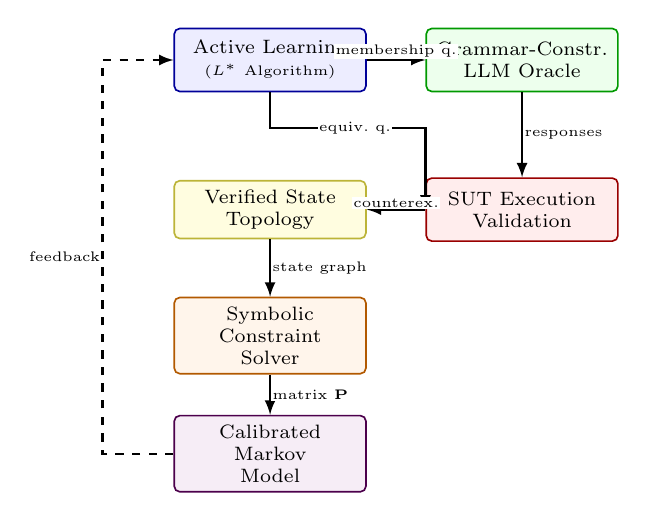
\begin{tikzpicture}[
          >=latex, font=\scriptsize,
          engine/.style={rectangle, draw=blue!60!black, rounded corners=2pt,
              fill=blue!7, minimum width=2.4cm, minimum height=0.8cm,
              text width=2.2cm, align=center, line width=0.6pt},
          oracle/.style={rectangle, draw=green!60!black, rounded corners=2pt,
              fill=green!7, minimum width=2.4cm, minimum height=0.8cm,
              text width=2.2cm, align=center, line width=0.6pt},
          sut/.style={rectangle, draw=red!60!black, rounded corners=2pt,
              fill=red!7, minimum width=2.4cm, minimum height=0.8cm,
              text width=2.2cm, align=center, line width=0.6pt},
          topo/.style={rectangle, draw=yellow!70!black, rounded corners=2pt,
              fill=yellow!12, minimum width=2.4cm, minimum height=0.7cm,
              text width=2.2cm, align=center, line width=0.6pt},
          solver/.style={rectangle, draw=orange!70!black, rounded corners=2pt,
              fill=orange!8, minimum width=2.4cm, minimum height=0.8cm,
              text width=2.2cm, align=center, line width=0.6pt},
          outnode/.style={rectangle, draw=violet!60!black, rounded corners=2pt,
              fill=violet!7, minimum width=2.4cm, minimum height=0.8cm,
              text width=2.2cm, align=center, line width=0.6pt},
          arr/.style={->, thick},
          darr/.style={->, thick, dashed},
          lbl/.style={font=\tiny, fill=white, inner sep=0.5pt}
      ]
      \node[engine]  (ale)    at (0,   0)    {Active Learning\\{\tiny ($L^*$ Algorithm)}};
      \node[oracle]  (oracle) at (3.2, 0)    {Grammar-Constr.\\LLM Oracle};
      \node[sut]     (sut)    at (3.2,-1.9)  {SUT Execution\\Validation};
      \node[topo]    (topo)   at (0,  -1.9)  {Verified State\\Topology};
      \node[solver]  (solver) at (0,  -3.5)  {Symbolic Constraint\\Solver};
      \node[outnode] (out)    at (0,  -5.0)  {Calibrated Markov\\Model};
      \draw[arr] (ale.east) -- node[lbl,above] {membership q.} (oracle.west);
      \draw[arr] (oracle.south) -- node[lbl,right] {responses} (sut.north);
      \draw[arr] (ale.south) -- ++(0,-0.45) -| node[lbl,right,pos=0.15] {equiv.\ q.} (sut.west);
      \draw[arr] (sut.west) -- node[lbl,above] {counterex.} (topo.east);
      \draw[arr] (topo.south) -- node[lbl,right] {state graph} (solver.north);
      \draw[arr] (solver.south) -- node[lbl,right] {matrix $\mathbf{P}$} (out.north);
      \draw[darr] (out.west) -- ++(-0.9,0) |- node[lbl,left,pos=0.25] {feedback} (ale.west);
      \end{tikzpicture}
  \end{columns}
\end{frame}

\begin{frame}{Component 1: Progress-Feasibility Dual Memory}
  \begin{columns}[T]
    \column{0.48\textwidth}
      \begin{exampleblock}{\pos{Neural Progress Memory}}
        Fine-tuned LLM parses NL requirements, drafts semantic flow graph.
        Captures \emph{what}: candidate states, events, transitions.
      \end{exampleblock}
    \column{0.48\textwidth}
      \begin{exampleblock}{\pos{Symbolic Feasibility Memory}}
        Rule-based engine enforces invariants, preconditions, transition guards.
        Ensures \emph{how}: reachable, deterministic, contradiction-free.
      \end{exampleblock}
  \end{columns}
  \vspace{0.5em}
  \textbf{Result:} topology is both \HL{semantically plausible} and \HL{mathematically sound}.\\
  Avoids the end-to-end neural failure mode: syntactically valid yet logically inconsistent models.
\end{frame}

\begin{frame}{Component 2: $L^*$ Active Automata Learning with LLM Oracle}
  \textbf{Two query types:}
  \begin{columns}[T]
    \column{0.48\textwidth}
      \begin{block}{Membership Queries}
        ``Does SUT accept input sequence $\sigma \in \Sigma^*$?''\\[4pt]
        Oracle vocabulary restricted to $\{\texttt{Yes},\, \texttt{No},\, \texttt{Unsure}\}$\\
        Eliminates hallucinated / malformed responses.
      \end{block}
    \column{0.48\textwidth}
      \begin{block}{Equivalence Queries}
        ``Is hypothesis automaton $\mathcal{H}$ equivalent to the target?''\\[4pt]
        Resolved by SUT execution. Counterexamples refine $\mathcal{H}$ iteratively.
      \end{block}
  \end{columns}
  \vspace{0.4em}
  \textbf{Convergence on AV benchmark:}
  \begin{itemize}
    \item \pos{94\%} of membership queries resolved directly by oracle
    \item \pos{6\%} escalated to SUT execution
    \item \texttt{Unsure} rate: 0\% on AV benchmark
  \end{itemize}
\end{frame}

\begin{frame}{Component 3 \& 4: Hierarchical Modeling + Convex Optimization}
  \begin{columns}[T]
    \column{0.48\textwidth}
      \textbf{Hierarchical Model (C3)}\\[4pt]
      \textbf{Upper:} higher-order Markov chain for frequent, path-dependent sequences:
      \[ P(s_{t+1} \mid s_t, s_{t-1}, \ldots, s_{t-k+1}) \]
      \textbf{Lower:} first-order chain for rare/exception paths:
      \[ P(s_{t+1} \mid s_t) \]
      Prevents state-space explosion while preserving fidelity.
    \column{0.48\textwidth}
      \textbf{Convex Optimization (C4)}\\[4pt]
      LLM extracts comparative constraints, e.g.:\\
      $P(\texttt{checkout} \mid \texttt{cart}) > P(\texttt{browse} \mid \texttt{cart})$\\[4pt]
      Solver enforces row-stochasticity + domain constraints:
      \[ \mathbf{P}^{*} = \arg\min_{\mathbf{P} \in \mathcal{C}}\; \mathcal{L}(\mathbf{P}) \]
      Maximum-entropy regularization avoids unjustified bias.
  \end{columns}
\end{frame}

% ─── SECTION 4: EVALUATION ───────────────────────────────────────────────────
\section{Empirical Evaluation}

\begin{frame}{RQ1: Extraction Accuracy — State \& Transition F1}
  \vspace{0.3em}
  \begin{center}
  \small
  \begin{tabular}{l ccc c}
    \toprule
    \textbf{Strategy} & \textbf{State F1} & \textbf{Trans.\ F1} & \textbf{System F1} \\
    \midrule
    Single-Prompt (GPT-4o)      & 0.80 & 0.54 & 0.543 \\
    Hybrid SMF (GPT-4o)         & 0.858 & 0.649 & 0.656 \\
    Single-Prompt (Claude 3.5)  & 0.90 & 0.75 & 0.795 \\
    \midrule
    \textbf{NeSy-MBST (ours)}   & \textbf{0.945} & \textbf{0.895} & \textbf{0.9125} \\
    \midrule
    \multicolumn{4}{l}{\small\textcolor{neutral}{Safety-critical threshold: $F_1 \geq 0.90$}} \\
    \bottomrule
  \end{tabular}
  \end{center}
  \vspace{0.4em}
  \begin{columns}[T]
    \column{0.55\textwidth}
      \textbf{Key findings:}
      \begin{itemize}
        \item \pos{+39.1\%} over best GPT-4o multi-frame strategy
        \item \pos{+14.8\%} over best single-model baseline
        \item First method to exceed 0.90 safety-critical threshold
      \end{itemize}
    \column{0.42\textwidth}
      \begin{exampleblock}{}
        \centering Symbolic verification loop\\
        converts recall-limited generation\\
        into \HL{verification-guided completion}
      \end{exampleblock}
  \end{columns}
\end{frame}

\begin{frame}{RQ2: Operational Coverage — E-Commerce Benchmark}
  \vspace{0.2em}
  \begin{center}
  \small
  \begin{tabular}{l r r c c l}
    \toprule
    \textbf{Model} & \textbf{States} & \textbf{Trans.} & \textbf{Req.\ Cov.} & \textbf{Tr.\ Cov.} & \textbf{Time} \\
    \midrule
    User  & 24 & 112 & \pos{100\%} & \pos{100\%} & 1\,m 48\,s \\
    Admin & 42 & 218 & \pos{100\%} & \pos{100\%} & 5\,m 49\,s \\
    \bottomrule
  \end{tabular}
  \end{center}
  \vspace{0.4em}
  \begin{itemize}
    \item Full model-coverage test generation in \HL{under 6 minutes} on models up to 42 states
    \item \pos{Sub-quadratic scaling}: Admin ($2\times$ complexity) requires only $3.2\times$ time
    \item NeSy-MBST baseline: 50\% transition coverage $\Rightarrow$ \pos{+35.7 pp gain}
    \item $\leq 3$ human-in-the-loop interventions per model in practice
  \end{itemize}
\end{frame}

\begin{frame}{RQ3: Statistical Fidelity — Jensen–Shannon Divergence}
  \begin{columns}[T]
    \column{0.52\textwidth}
      \textbf{Validation metrics:}
      \begin{itemize}
        \item \textbf{JSD} measures aggregate activity marginal divergence
        \item \textbf{Frobenius distance} measures entry-wise matrix deviation
      \end{itemize}
      \vspace{0.5em}
      \begin{center}
      \small
      \begin{tabular}{l c c}
        \toprule
        \textbf{Metric} & \textbf{Value} \\
        \midrule
        Jensen–Shannon Divergence & \pos{0.0142} \\
        Frobenius Distance (norm.) & \pos{0.0841} \\
        \bottomrule
      \end{tabular}
      \end{center}
    \column{0.44\textwidth}
      \begin{exampleblock}{\HL{Interpretation}}
        JSD\,=\,0.012 confirms \pos{preserved operational test-allocation fidelity}.\\[6pt]
        Entropy-maximizing SLSQP solver vs.\ uncalibrated: JSD 0.157 $\to$ 0.012.\\
        A \HL{93\% reduction} in divergence.
      \end{exampleblock}
  \end{columns}
\end{frame}

% ─── SECTION 5: ABLATION ─────────────────────────────────────────────────────
\section{Ablation Study}

\begin{frame}{RQ4: Component Necessity — Ablation on AV CPS Benchmark}
  \vspace{0.2em}
  \begin{center}
  \scriptsize
  \begin{tabular}{l ccc cc cc r}
    \toprule
    & \multicolumn{3}{c}{\textbf{Structural F1}} & \multicolumn{2}{c}{\textbf{Prob.\ Fidelity}} & \multicolumn{2}{c}{\textbf{Coverage}} & \\
    \cmidrule(lr){2-4}\cmidrule(lr){5-6}\cmidrule(lr){7-8}
    \textbf{Condition} & \textbf{St.F1} & \textbf{Tr.F1} & \textbf{Sys.F1} & \textbf{JSD} & \textbf{Frob} & \textbf{St.} & \textbf{Tr.} & \textbf{Time} \\
    \midrule
    A — Pure-Neural           & 1.00 & 0.783 & 0.904 & 0.157 & 0.163 & 55.6\% & 50.0\% & 2.35s \\
    B — +Symbolic Loop        & 1.00 & \pos{0.963} & \pos{0.982} & \pos{0.012} & \pos{0.084} & \pos{88.9\%} & \pos{85.7\%} & 10.66s \\
    C — +Convex Optimizer     & 1.00 & 0.963 & 0.982 & 0.012 & 0.084 & 88.9\% & 85.7\% & 2.13s \\
    \textbf{D — Full NeSy-MBST} & \textbf{1.00} & \textbf{0.963} & \textbf{0.982} & \textbf{0.012} & \textbf{0.084} & \textbf{88.9\%} & \textbf{85.7\%} & 10.59s \\
    \bottomrule
  \end{tabular}
  \end{center}
  \vspace{0.3em}
  \begin{itemize}
    \item \textbf{A$\to$B} (\pos{Symbolic loop}): Tr.F1 $0.783 \to 0.963$; JSD $0.157 \to 0.012$; coverage $+33\,$pp
    \item \textbf{B$\to$C} (\pos{Convex optimizer}): structural F1/coverage unchanged; governs probabilistic calibration
    \item \textbf{C$\to$D} (Closed-loop): marginal JSD $\Delta{-0.0002}$; value accumulates over extended campaigns
  \end{itemize}
\end{frame}

\begin{frame}{Ablation Insight: Two Orthogonal Failure Modes}
  \begin{columns}[T]
    \column{0.48\textwidth}
      \begin{exampleblock}{\pos{Symbolic Loop} — Structural Errors}
        Corrects wrong topology:\\
        unreachable states, missing transitions,\\
        dangling edges.\\[6pt]
        Measured by: \textbf{F1, Coverage}
      \end{exampleblock}
    \column{0.48\textwidth}
      \begin{exampleblock}{\pos{Convex Optimizer} — Calibration Errors}
        Corrects wrong probability mass distribution:\\
        miscalibrated row-stochastic matrix.\\[6pt]
        Measured by: \textbf{JSD, Frobenius distance}
      \end{exampleblock}
  \end{columns}
  \vspace{0.6em}
  \begin{center}
    \HL{The two components address orthogonal failure modes — both are necessary.}\\[4pt]
    \small High F1 $\not\Rightarrow$ low JSD. \quad Low JSD $\not\Rightarrow$ high coverage. \quad These three axes are independent.
  \end{center}
\end{frame}

% ─── SECTION 6: CONCLUSION ───────────────────────────────────────────────────
\section{Conclusion}

\begin{frame}{Summary of Results}
  \begin{center}
  \begin{tabular}{l l l}
    \toprule
    \textbf{RQ} & \textbf{Question} & \textbf{Result} \\
    \midrule
    RQ1 & Structural fidelity & \pos{F1\,=\,0.9125} (exceeds 0.90 threshold) \\
    RQ2 & Fault-detection coverage & \pos{85.7\%} transition cov.\ vs.\ 50\% baseline \\
    RQ3 & Probabilistic calibration & \pos{JSD\,=\,0.012}; 93\% divergence reduction \\
    RQ4 & Component necessity & Symbolic loop (structure); solver (calibration) \\
    \bottomrule
  \end{tabular}
  \end{center}
  \vspace{0.4em}
  \begin{block}{Core Finding}
    NeSy-MBST \HL{eliminates the manual modelling bottleneck} without compromising statistical rigour demanded by safety-critical CPS.
  \end{block}
\end{frame}

\begin{frame}{Adoption Guidelines}
  \begin{enumerate}
    \item \textbf{Grammar-constrained oracles} — restrict LLM output to $\{\texttt{Yes},\texttt{No},\texttt{Unsure}\}$; prevents hallucinated artefacts
    \item \textbf{Symbolic verification loop before probability assignment} — +35.7\,pp transition coverage, 93\% JSD reduction
    \item \textbf{Convex optimization, not direct LLM output} — JSD 0.157 $\to$ 0.012 (SLSQP entropy-maximizing)
    \item \textbf{Hierarchical multi-tier models} — controls state-space explosion for large systems
    \item \textbf{Closed-loop telemetry recalibration} — prevents model drift as usage patterns evolve
  \end{enumerate}
  \vspace{0.4em}
  \begin{center}
    \HL{LLM augmentation of formal test-model generation should be standard engineering practice,}\\
    \small provided: (1) grammar-constrained output + symbolic loop; (2) solver-assigned probabilities.
  \end{center}
\end{frame}

\begin{frame}{Limitations \& Future Work}
  \begin{columns}[T]
    \column{0.48\textwidth}
      \textbf{\con{Current scope:}}
      \begin{itemize}
        \item Two domains: AV CPS + e-commerce
        \item Models up to 42 states
        \item Single-author ground-truth annotation
        \item No direct fault-seeding measurement
      \end{itemize}
    \column{0.48\textwidth}
      \textbf{\pos{Next steps:}}
      \begin{itemize}
        \item Fault-seeding experiments on industrial SUTs
        \item Generalise: telecom, medical device, ISO\,26262
        \item Multi-annotator inter-rater reliability protocol
        \item Three-valued oracle at scale: convergence characterization
      \end{itemize}
  \end{columns}
  \vspace{0.4em}
  \begin{center}
    \small Replication package: \texttt{https://github.com/nathangtg/llm-mbst-research}\\
    \texttt{python run\_ablation.py} (seed\,42, Azure OpenAI backend)
  \end{center}
\end{frame}

% ─── REFERENCES ──────────────────────────────────────────────────────────────
\begin{frame}{References}
  \begin{thebibliography}{9}
    \small
    \bibitem{whittaker1993markov} J.\,A.\ Whittaker \& M.\,G.\ Thomason, ``A Markov chain model for statistical software testing,'' \textit{IEEE Trans.\ Softw.\ Eng.}, 1994.
    \bibitem{angluin1987} D.\ Angluin, ``Learning regular sets from queries and counterexamples,'' \textit{Information and Computation}, 75(2), 1987.
    \bibitem{llm_state_machine_frameworks} O.\ Abdulkarim et al., ``LLM-Assisted State Machine Frameworks for MBT,'' 2024.
    \bibitem{boehr_constraints} R.\ Boehr et al., ``Operational profile constraint extraction,'' \textit{ICST}, 2023.
    \bibitem{garcez2023neurosymbolic} A.\ Garcez \& L.\ Lamb, ``Neurosymbolic AI: The 3rd wave,'' \textit{AIJ}, 2023.
    \bibitem{taxonomy_mbt} M.\ Utting \& B.\ Legeard, \textit{Practical Model-Based Testing: A tools approach}. Elsevier, 2007.
  \end{thebibliography}
\end{frame}

% ─── THANK YOU ───────────────────────────────────────────────────────────────
\begin{frame}
  \begin{center}
    \vspace{1em}
    {\Large \textbf{Thank You}}\\[1em]
    {\large Questions?}\\[2em]
    \small
    Nathan G.\ \quad \texttt{nathan.n@imail.sunway.edu.my}\\[0.5em]
    \url{https://github.com/nathangtg/llm-mbst-research}
  \end{center}
\end{frame}

% ─── BACKUP SLIDES ───────────────────────────────────────────────────────────
\appendix

\begin{frame}{Backup Slides}
  \begin{center}
    \textit{Backup slides for anticipated questions}
  \end{center}
\end{frame}

\begin{frame}{Backup: Mathematical Formulation — Stochastic Constraints}
  \textbf{Valid Markov chain usage model must satisfy:}
  \begin{align}
    0 &\leq p_{ij} \leq 1 \quad \forall\, i,j \label{eq:prob_bounds} \\
    \sum_{j} p_{ij} &= 1 \quad \forall\, i \label{eq:row_stochastic}
  \end{align}
  \textbf{Convex optimization formulation:}
  \[ \mathbf{P}^{*} = \arg\min_{\mathbf{P} \in \mathcal{C}}\; \mathcal{L}(\mathbf{P}) \]
  where $\mathcal{C}$ is the feasible set (stochastic + domain constraints), and $\mathcal{L}(\cdot)$ is the maximum-entropy regularization objective.\\[6pt]
  Decouples: LLM for constraint \emph{extraction} (NL task); solver for constraint \emph{resolution} (math task).
\end{frame}

\begin{frame}{Backup: $L^*$ Convergence \& Oracle Design}
  \begin{itemize}
    \item Classic Angluin $L^*$ convergence guarantee: holds for consistent binary oracles
    \item Three-valued oracle ($\{\texttt{Yes},\texttt{No},\texttt{Unsure}\}$): empirically verified convergence on AV benchmark
    \item \texttt{Unsure} escalation: $\to$ human expert OR $\to$ SUT execution for empirical resolution
    \item Grammar-constrained output schema: eliminates hallucinated/malformed oracle responses
  \end{itemize}
  \vspace{0.3em}
  \begin{block}{Formal target}
    Learned structure $\mathcal{A} = (Q,\Sigma,\delta,q_0)$ is the \emph{support topology} of the target Markov chain, not a classical DFA accepting language. Membership oracle answers reachability queries.
  \end{block}
\end{frame}

\begin{frame}{Backup: AV CPS System-Under-Test Architecture}
  \begin{center}
  \scalebox{0.82}{%
  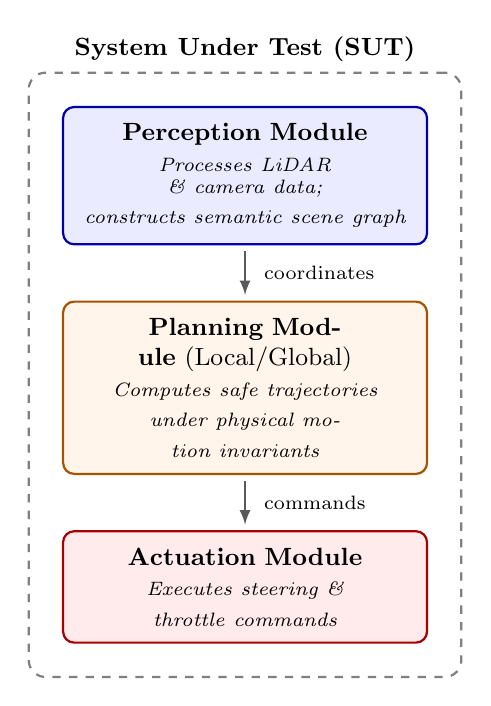
\begin{tikzpicture}[
      >=latex, font=\small,
      modblue/.style={rectangle, draw=blue!65!black, thick, rounded corners=4pt,
          fill=blue!8, minimum width=4.6cm, text width=4.2cm,
          align=center, inner sep=6pt},
      modorange/.style={rectangle, draw=orange!65!black, thick, rounded corners=4pt,
          fill=orange!8, minimum width=4.6cm, text width=4.2cm,
          align=center, inner sep=6pt},
      modred/.style={rectangle, draw=red!65!black, thick, rounded corners=4pt,
          fill=red!8, minimum width=4.6cm, text width=4.2cm,
          align=center, inner sep=6pt},
      flow/.style={->, thick, draw=black!65, shorten >=2pt, shorten <=2pt},
      arrlbl/.style={font=\scriptsize, fill=white, inner sep=1.5pt, midway, right=5pt}
  ]
  \node[modblue] (percep) {%
      \textbf{Perception Module}\\[3pt]
      {\scriptsize\itshape Processes LiDAR \& camera data;\\constructs semantic scene graph}};
  \node[modorange, below=0.7cm of percep] (plan) {%
      \textbf{Planning Module} {\small (Local/Global)}\\[3pt]
      {\scriptsize\itshape Computes safe trajectories\\under physical motion invariants}};
  \node[modred, below=0.7cm of plan] (act) {%
      \textbf{Actuation Module}\\[3pt]
      {\scriptsize\itshape Executes steering \&\\throttle commands}};
  \draw[flow] (percep.south) -- node[arrlbl] {coordinates} (plan.north);
  \draw[flow] (plan.south)   -- node[arrlbl] {commands}    (act.north);
  \node[draw=black!50, dashed, thick, rounded corners=6pt, inner sep=12pt,
        fit=(percep)(plan)(act),
        label={[font=\small\bfseries]above:System Under Test (SUT)}] {};
  \end{tikzpicture}}
  \end{center}
\end{frame}

\begin{frame}{Backup: Metric Decomposition}
  \begin{center}
  \begin{tabular}{l l l}
    \toprule
    \textbf{Metric} & \textbf{What it measures} & \textbf{Orthogonal to} \\
    \midrule
    F1 (state/transition) & Structural correctness & JSD, Coverage \\
    JSD / Frobenius dist. & Probabilistic fidelity & F1, Coverage \\
    Transition coverage & Test suite completeness & F1, JSD \\
    \bottomrule
  \end{tabular}
  \end{center}
  \vspace{0.5em}
  \begin{itemize}
    \item High F1 $\not\Rightarrow$ low JSD: correct topology, wrong probability mass
    \item Low JSD $\not\Rightarrow$ high coverage: accurate probabilities, test generator fails to reach rare states
    \item All three axes must be evaluated independently for a complete picture of MBST quality
  \end{itemize}
\end{frame}

\end{document}
